\documentclass[]{article}
\usepackage{lmodern}
\usepackage{amssymb,amsmath}
\usepackage{ifxetex,ifluatex}
\usepackage{fixltx2e} % provides \textsubscript
\ifnum 0\ifxetex 1\fi\ifluatex 1\fi=0 % if pdftex
  \usepackage[T1]{fontenc}
  \usepackage[utf8]{inputenc}
\else % if luatex or xelatex
  \ifxetex
    \usepackage{mathspec}
  \else
    \usepackage{fontspec}
  \fi
  \defaultfontfeatures{Ligatures=TeX,Scale=MatchLowercase}
\fi
% use upquote if available, for straight quotes in verbatim environments
\IfFileExists{upquote.sty}{\usepackage{upquote}}{}
% use microtype if available
\IfFileExists{microtype.sty}{%
\usepackage{microtype}
\UseMicrotypeSet[protrusion]{basicmath} % disable protrusion for tt fonts
}{}
\usepackage[margin=1in]{geometry}
\usepackage{hyperref}
\hypersetup{unicode=true,
            pdftitle={Agenda Bias},
            pdfborder={0 0 0},
            breaklinks=true}
\urlstyle{same}  % don't use monospace font for urls
\usepackage{color}
\usepackage{fancyvrb}
\newcommand{\VerbBar}{|}
\newcommand{\VERB}{\Verb[commandchars=\\\{\}]}
\DefineVerbatimEnvironment{Highlighting}{Verbatim}{commandchars=\\\{\}}
% Add ',fontsize=\small' for more characters per line
\usepackage{framed}
\definecolor{shadecolor}{RGB}{248,248,248}
\newenvironment{Shaded}{\begin{snugshade}}{\end{snugshade}}
\newcommand{\KeywordTok}[1]{\textcolor[rgb]{0.13,0.29,0.53}{\textbf{#1}}}
\newcommand{\DataTypeTok}[1]{\textcolor[rgb]{0.13,0.29,0.53}{#1}}
\newcommand{\DecValTok}[1]{\textcolor[rgb]{0.00,0.00,0.81}{#1}}
\newcommand{\BaseNTok}[1]{\textcolor[rgb]{0.00,0.00,0.81}{#1}}
\newcommand{\FloatTok}[1]{\textcolor[rgb]{0.00,0.00,0.81}{#1}}
\newcommand{\ConstantTok}[1]{\textcolor[rgb]{0.00,0.00,0.00}{#1}}
\newcommand{\CharTok}[1]{\textcolor[rgb]{0.31,0.60,0.02}{#1}}
\newcommand{\SpecialCharTok}[1]{\textcolor[rgb]{0.00,0.00,0.00}{#1}}
\newcommand{\StringTok}[1]{\textcolor[rgb]{0.31,0.60,0.02}{#1}}
\newcommand{\VerbatimStringTok}[1]{\textcolor[rgb]{0.31,0.60,0.02}{#1}}
\newcommand{\SpecialStringTok}[1]{\textcolor[rgb]{0.31,0.60,0.02}{#1}}
\newcommand{\ImportTok}[1]{#1}
\newcommand{\CommentTok}[1]{\textcolor[rgb]{0.56,0.35,0.01}{\textit{#1}}}
\newcommand{\DocumentationTok}[1]{\textcolor[rgb]{0.56,0.35,0.01}{\textbf{\textit{#1}}}}
\newcommand{\AnnotationTok}[1]{\textcolor[rgb]{0.56,0.35,0.01}{\textbf{\textit{#1}}}}
\newcommand{\CommentVarTok}[1]{\textcolor[rgb]{0.56,0.35,0.01}{\textbf{\textit{#1}}}}
\newcommand{\OtherTok}[1]{\textcolor[rgb]{0.56,0.35,0.01}{#1}}
\newcommand{\FunctionTok}[1]{\textcolor[rgb]{0.00,0.00,0.00}{#1}}
\newcommand{\VariableTok}[1]{\textcolor[rgb]{0.00,0.00,0.00}{#1}}
\newcommand{\ControlFlowTok}[1]{\textcolor[rgb]{0.13,0.29,0.53}{\textbf{#1}}}
\newcommand{\OperatorTok}[1]{\textcolor[rgb]{0.81,0.36,0.00}{\textbf{#1}}}
\newcommand{\BuiltInTok}[1]{#1}
\newcommand{\ExtensionTok}[1]{#1}
\newcommand{\PreprocessorTok}[1]{\textcolor[rgb]{0.56,0.35,0.01}{\textit{#1}}}
\newcommand{\AttributeTok}[1]{\textcolor[rgb]{0.77,0.63,0.00}{#1}}
\newcommand{\RegionMarkerTok}[1]{#1}
\newcommand{\InformationTok}[1]{\textcolor[rgb]{0.56,0.35,0.01}{\textbf{\textit{#1}}}}
\newcommand{\WarningTok}[1]{\textcolor[rgb]{0.56,0.35,0.01}{\textbf{\textit{#1}}}}
\newcommand{\AlertTok}[1]{\textcolor[rgb]{0.94,0.16,0.16}{#1}}
\newcommand{\ErrorTok}[1]{\textcolor[rgb]{0.64,0.00,0.00}{\textbf{#1}}}
\newcommand{\NormalTok}[1]{#1}
\usepackage{graphicx,grffile}
\makeatletter
\def\maxwidth{\ifdim\Gin@nat@width>\linewidth\linewidth\else\Gin@nat@width\fi}
\def\maxheight{\ifdim\Gin@nat@height>\textheight\textheight\else\Gin@nat@height\fi}
\makeatother
% Scale images if necessary, so that they will not overflow the page
% margins by default, and it is still possible to overwrite the defaults
% using explicit options in \includegraphics[width, height, ...]{}
\setkeys{Gin}{width=\maxwidth,height=\maxheight,keepaspectratio}
\IfFileExists{parskip.sty}{%
\usepackage{parskip}
}{% else
\setlength{\parindent}{0pt}
\setlength{\parskip}{6pt plus 2pt minus 1pt}
}
\setlength{\emergencystretch}{3em}  % prevent overfull lines
\providecommand{\tightlist}{%
  \setlength{\itemsep}{0pt}\setlength{\parskip}{0pt}}
\setcounter{secnumdepth}{0}
% Redefines (sub)paragraphs to behave more like sections
\ifx\paragraph\undefined\else
\let\oldparagraph\paragraph
\renewcommand{\paragraph}[1]{\oldparagraph{#1}\mbox{}}
\fi
\ifx\subparagraph\undefined\else
\let\oldsubparagraph\subparagraph
\renewcommand{\subparagraph}[1]{\oldsubparagraph{#1}\mbox{}}
\fi

%%% Use protect on footnotes to avoid problems with footnotes in titles
\let\rmarkdownfootnote\footnote%
\def\footnote{\protect\rmarkdownfootnote}

%%% Change title format to be more compact
\usepackage{titling}

% Create subtitle command for use in maketitle
\newcommand{\subtitle}[1]{
  \posttitle{
    \begin{center}\large#1\end{center}
    }
}

\setlength{\droptitle}{-2em}

  \title{Agenda Bias}
    \pretitle{\vspace{\droptitle}\centering\huge}
  \posttitle{\par}
  \subtitle{Control for topical prevalence}
  \author{}
    \preauthor{}\postauthor{}
    \date{}
    \predate{}\postdate{}
  

\begin{document}
\maketitle

To allow for an operationalization of agenda bias, I use parties'
campaign communication as an approximation of the potential universe of
news stories (D'Alessio \& Allen, 2000; Eberl, 2017). I compare the
policy issues addressed in campaign communication (i.e., the party
agenda) with the policy issues the parties address in media coverage
(i.e., the mediated party agenda).

To discover the latent topics in the corpus of press releases (1.942)
and news articles (11.880), a structural topic modeling (STM) developed
by
\href{https://scholar.princeton.edu/sites/default/files/bstewart/files/a_model_of_text_for_experimentation_in_the_social_sciences.pdf}{Roberts
(2016)} is applied. The STM is an unsupervised machine learning approach
that models topics as multinomial distributions of words and documents
as multinomial distributions of topics, allowing to incorporate external
variables that effect both, topical content and topical prevalence.

\section{Structural Topic Model}\label{structural-topic-model}

\subsection{Combine press release with news
articles}\label{combine-press-release-with-news-articles}

\begin{Shaded}
\begin{Highlighting}[]
\KeywordTok{library}\NormalTok{(stm)}
\KeywordTok{library}\NormalTok{(tidyverse)}
\KeywordTok{library}\NormalTok{(dplyr)}

\KeywordTok{rm}\NormalTok{(}\DataTypeTok{list =} \KeywordTok{ls}\NormalTok{())}
\KeywordTok{load}\NormalTok{(}\StringTok{"../output/pressReleases.Rda"}\NormalTok{)}
\KeywordTok{load}\NormalTok{(}\StringTok{"../output/data_step2.Rda"}\NormalTok{)}

\NormalTok{btw }\OperatorTok
\StringTok{  }\KeywordTok{mutate}\NormalTok{(}\DataTypeTok{date =} \KeywordTok{as.Date}\NormalTok{(date),}
         \DataTypeTok{type =} \StringTok{"news"}\NormalTok{,}
         \DataTypeTok{source =}\NormalTok{ medium }
\NormalTok{         ) }\OperatorTok
\StringTok{  }\KeywordTok{bind_rows}\NormalTok{(.,pressReleases) ->}\StringTok{ }\NormalTok{model_df}
\end{Highlighting}
\end{Shaded}

\begin{Shaded}
\begin{Highlighting}[]
\NormalTok{model_df }\OperatorTok
\StringTok{  }\KeywordTok{ggplot}\NormalTok{(}\KeywordTok{aes}\NormalTok{(source, }\DataTypeTok{fill=}\NormalTok{type)) }\OperatorTok{+}
\StringTok{  }\KeywordTok{geom_bar}\NormalTok{(}\DataTypeTok{show.legend =}\NormalTok{ F) }\OperatorTok{+}
\StringTok{  }\KeywordTok{facet_wrap}\NormalTok{(}\OperatorTok{~}\NormalTok{type, }\DataTypeTok{scales =} \StringTok{"free"}\NormalTok{) }\OperatorTok{+}
\StringTok{  }\NormalTok{ggthemes}\OperatorTok{::}\KeywordTok{theme_igray}\NormalTok{() }\OperatorTok{+}
\StringTok{  }\NormalTok{ggthemes}\OperatorTok{::}\KeywordTok{scale_fill_economist}\NormalTok{() }\OperatorTok{+}
\StringTok{  }\KeywordTok{labs}\NormalTok{(}\DataTypeTok{title =} \StringTok{"Document distribution"}\NormalTok{, }\DataTypeTok{y=}\OtherTok{NULL}\NormalTok{)}
\end{Highlighting}
\end{Shaded}

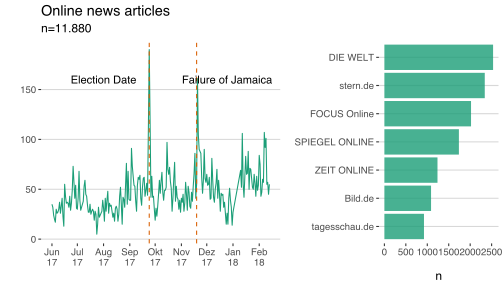
\includegraphics{agendaBias2_files/figure-latex/unnamed-chunk-2-1.pdf}

\subsection{Build Corpus}\label{build-corpus}

I included the document source as a control for the topical topical
prevalenc. Thus, I assume that the distribution of topics depends on the
source. The number of topics is set to 40.

\subsection{Run Model}\label{run-model}

\subsection{Results}\label{results}

\begin{Shaded}
\begin{Highlighting}[]
\KeywordTok{library}\NormalTok{(stm)}
\KeywordTok{library}\NormalTok{(tidyverse)}

\KeywordTok{rm}\NormalTok{(}\DataTypeTok{list =} \KeywordTok{ls}\NormalTok{())}
\KeywordTok{source}\NormalTok{(}\StringTok{"func/functions.R"}\NormalTok{)}
\KeywordTok{load}\NormalTok{(}\StringTok{"../output/models/finalmodel_40.RData"}\NormalTok{)}

\NormalTok{model_df <-}\StringTok{ }\NormalTok{model_df }\OperatorTok
\StringTok{  }\KeywordTok{mutate}\NormalTok{(}\DataTypeTok{doc_index =} \KeywordTok{as.numeric}\NormalTok{(}\KeywordTok{rownames}\NormalTok{(.)))}
\end{Highlighting}
\end{Shaded}

\begin{Shaded}
\begin{Highlighting}[]
\NormalTok{## Label topics}
\NormalTok{labels <-}\StringTok{ }\KeywordTok{labelTopics}\NormalTok{(stmOut)}

\NormalTok{topics.df <-}\StringTok{ }\KeywordTok{as.data.frame}\NormalTok{(labels}\OperatorTok{$}\NormalTok{prob) }\OperatorTok
\StringTok{  }\KeywordTok{transmute}\NormalTok{(}\DataTypeTok{topic =} \KeywordTok{as.numeric}\NormalTok{(}\KeywordTok{rownames}\NormalTok{(.)),}
            \DataTypeTok{topic_name =} \KeywordTok{paste}\NormalTok{(}\StringTok{"Topic"}\NormalTok{,}\KeywordTok{as.character}\NormalTok{(topic),}\StringTok{":"}\NormalTok{,V1,V2,V3,V4))}
\end{Highlighting}
\end{Shaded}

\subsubsection{Topic frequency}\label{topic-frequency}

In order to get an initial overview of the results, the figure below
displays the topics ordered by their expected frequency across the
corpus. The four most frequent words in each topic are used as a label
for that topic.

\begin{Shaded}
\begin{Highlighting}[]
\NormalTok{overall_freq }\OperatorTok
\StringTok{  }\KeywordTok{ggplot}\NormalTok{(}\KeywordTok{aes}\NormalTok{(}\KeywordTok{reorder}\NormalTok{(topic_name, }\OperatorTok{-}\NormalTok{order), frequency)) }\OperatorTok{+}
\StringTok{  }\KeywordTok{geom_col}\NormalTok{(}\DataTypeTok{alpha =} \FloatTok{0.7}\NormalTok{) }\OperatorTok{+}
\StringTok{  }\KeywordTok{coord_flip}\NormalTok{() }\OperatorTok{+}
\StringTok{  }\NormalTok{ggthemes}\OperatorTok{::}\KeywordTok{theme_igray}\NormalTok{() }\OperatorTok{+}
\StringTok{  }\KeywordTok{labs}\NormalTok{(}\DataTypeTok{x=}\OtherTok{NULL}\NormalTok{, }\DataTypeTok{y=}\OtherTok{NULL}\NormalTok{, }\DataTypeTok{title=}\StringTok{"Expected Frequency of Topics"}\NormalTok{) }
\end{Highlighting}
\end{Shaded}

\includegraphics{agendaBias2_files/figure-latex/unnamed-chunk-8-1.pdf}

\subsubsection{Measure Agendas}\label{measure-agendas}

\begin{Shaded}
\begin{Highlighting}[]
\NormalTok{theta <-}\StringTok{ }\KeywordTok{as.data.frame}\NormalTok{(stmOut}\OperatorTok{$}\NormalTok{theta) }\OperatorTok\StringTok{ }\CommentTok{# get all theta values for echt document}
\StringTok{  }
\StringTok{  }\KeywordTok{mutate}\NormalTok{(}\DataTypeTok{doc_index =} \KeywordTok{as.numeric}\NormalTok{(}\KeywordTok{rownames}\NormalTok{(.))) }\OperatorTok
\StringTok{  }\CommentTok{# convert to long format}
\StringTok{  }\KeywordTok{gather}\NormalTok{(topic, theta, V1}\OperatorTok{:}\NormalTok{V40) }\OperatorTok
\StringTok{  }\KeywordTok{mutate}\NormalTok{(}\DataTypeTok{topic =} \KeywordTok{as.numeric}\NormalTok{(}\KeywordTok{gsub}\NormalTok{(}\StringTok{"V"}\NormalTok{,}\StringTok{""}\NormalTok{,topic))) }\OperatorTok
\StringTok{  }
\StringTok{  }\CommentTok{# join with topic df}
\StringTok{  }\KeywordTok{left_join}\NormalTok{(., topics.df, }\DataTypeTok{by=}\StringTok{"topic"}\NormalTok{) }\OperatorTok
\StringTok{  }
\StringTok{  }\CommentTok{# join with model_df}
\StringTok{  }\KeywordTok{left_join}\NormalTok{(., model_df }\OperatorTok\StringTok{ }
\StringTok{              }\KeywordTok{select}\NormalTok{(date,type,source,doc_index,title_text), }\DataTypeTok{by=}\StringTok{"doc_index"}\NormalTok{)}
\end{Highlighting}
\end{Shaded}

For each document, we have a distribution over all topics:

\begin{Shaded}
\begin{Highlighting}[]
\NormalTok{sample_doc <-}\StringTok{ }\KeywordTok{sample}\NormalTok{(}\KeywordTok{nrow}\NormalTok{(model_df),}\DecValTok{1}\NormalTok{)}

\CommentTok{# uncomment this to only select docs from press releases}
\CommentTok{#sample_doc <- theta %>% filter(type=="press") %>% sample_n(1) %>% select(doc_index)}
\CommentTok{#sample_doc <- sample_doc$doc_index}

\NormalTok{title <-}\StringTok{ }\NormalTok{model_df}\OperatorTok{$}\NormalTok{title[}\KeywordTok{which}\NormalTok{(model_df}\OperatorTok{$}\NormalTok{doc_index }\OperatorTok{==}\StringTok{ }\NormalTok{sample_doc)]}
\NormalTok{source <-}\StringTok{ }\NormalTok{model_df}\OperatorTok{$}\NormalTok{source[}\KeywordTok{which}\NormalTok{(model_df}\OperatorTok{$}\NormalTok{doc_index }\OperatorTok{==}\StringTok{ }\NormalTok{sample_doc)]}

\NormalTok{theta }\OperatorTok
\StringTok{  }\KeywordTok{filter}\NormalTok{(doc_index }\OperatorTok{==}\StringTok{ }\NormalTok{sample_doc) }\OperatorTok
\StringTok{  }\KeywordTok{select}\NormalTok{(doc_index, topic_name, theta) }\OperatorTok
\StringTok{  }\KeywordTok{ggplot}\NormalTok{(}\KeywordTok{aes}\NormalTok{(topic_name, theta)) }\OperatorTok{+}
\StringTok{  }\KeywordTok{geom_col}\NormalTok{() }\OperatorTok{+}
\StringTok{  }\KeywordTok{ylim}\NormalTok{(}\KeywordTok{c}\NormalTok{(}\DecValTok{0}\NormalTok{,}\DecValTok{1}\NormalTok{)) }\OperatorTok{+}
\StringTok{  }\KeywordTok{coord_flip}\NormalTok{() }\OperatorTok{+}
\StringTok{  }\NormalTok{ggthemes}\OperatorTok{::}\KeywordTok{theme_igray}\NormalTok{() }\OperatorTok{+}
\StringTok{  }\KeywordTok{labs}\NormalTok{(}\DataTypeTok{title =} \KeywordTok{paste}\NormalTok{(}\StringTok{"Topic distribution of document"}\NormalTok{,sample_doc),}
       \DataTypeTok{subtitle =} \KeywordTok{paste0}\NormalTok{(}\StringTok{"Source: "}\NormalTok{,source,}\StringTok{"}\CharTok{\textbackslash{}n}\StringTok{Title: "}\NormalTok{, title),}
       \DataTypeTok{x =} \OtherTok{NULL}\NormalTok{, }\DataTypeTok{y =} \OtherTok{NULL}
\NormalTok{       )}
\end{Highlighting}
\end{Shaded}

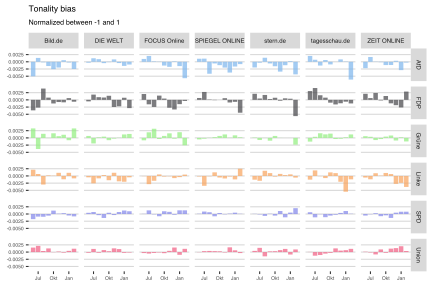
\includegraphics{agendaBias2_files/figure-latex/unnamed-chunk-10-1.pdf}

What is the document acutally about?

\begin{Shaded}
\begin{Highlighting}[]
\NormalTok{model_df }\OperatorTok
\StringTok{  }\KeywordTok{filter}\NormalTok{(doc_index }\OperatorTok{==}\StringTok{ }\NormalTok{sample_doc) }\OperatorTok
\StringTok{  }\KeywordTok{select}\NormalTok{(source, title_text) }\OperatorTok
\StringTok{  }\NormalTok{htmlTable}\OperatorTok{::}\KeywordTok{htmlTable}\NormalTok{()}
\end{Highlighting}
\end{Shaded}

source

title\_text

1

zeit.de

Bundeswehr: ``Afghanistan wird uns noch lange begleiten'' Die
internationalen Truppen hätten sich zu schnell aus Afghanistan zurück
gezogen, bemängelt Verteidigungsministerin von der Leyen. Sie fordert
einen ``langen Atem''.

Bundesverteidigungsministerin Ursula von der Leyen hat den Abzug der
internationalen Truppen aus Afghanistan in den vergangenen Jahren als zu
schnell kritisiert. Sie forderte einen ``langen Atem'' beim Einsatz am
Hindukusch. Die Zahl der internationalen Truppen sei mit dem Ende des
Isaf-Kampfeinsatzes 2014 zu schnell abgesenkt worden, sagte die
CDU-Politikerin bei einem Besuch der Soldaten im nordafghanischen
Masar-i-Scharif. Inzwischen habe die internationale Gemeinschaft aber
gelernt, dass sie mehr Geduld aufbringen müsse. ``Wir alle wissen, dass
die Sicherheitslage im Land nach wie vor angespannt ist''. Die Afghanen
brauchten weiter die Unterstützung, Beratung und die Ausbildung durch
die ausländischen Soldaten.

``Es gibt noch viel zu tun. Aber ich bin überzeugt, dass wir mit unserem
Engagement auf dem richtigen Weg sind'', sagte die Ministerin.
``Afghanistan wird uns noch lange begleiten.'' US-Präsident Donald Trump
hatte im Sommer die Aufstockung der US-Truppen angekündigt und damit
nach Jahren des Truppenabbaus eine Trendwende eingeleitet. Zu Hochzeiten
des Isaf-Kampfeinsatzes waren etwa 150.000 ausländische Soldaten am
Hindukusch im Einsatz. Aktuell sind es noch gut 17.000, unter ihnen
10.000 US-Amerikaner.

Deutschland hatte seine Truppen am Hindukusch 2016 wieder aufgestockt
und hat momentan knapp 1.000 Soldaten vor allem in Masar-i-Scharif und
Kabul stationiert. Die Bundeswehr ist damit der zweitgrößte
Truppensteller nach den USA. Aufgabe der deutschen Soldaten ist die
Beratung der einheimischen Sicherheitskräfte als Teil des Nato-Einsatzes
Resolute Support. Ein Teil der US-Soldaten dagegen ist abseits dieser
Mission weiter im Kampfeinsatz.

Mit Trumps Strategiewechsel verschärfte das US-Militär auch den Kampf
gegen die radikalislamischen Taliban. Die USA warfen in diesem Jahr drei
Mal so viele Bomben über Afghanistan ab wie 2016, US-Spezialkräfte
ziehen zudem routinemäßig mit afghanischen Elitetruppen in den Einsatz.
Hunderte Taliban wurden dabei getötet.

Seitennavigation Startseite

Agendas were measured in terms of percentage distributions across the 40
topics. For each source the average distribution of each topic is
calculated.

\begin{Shaded}
\begin{Highlighting}[]
\NormalTok{topicmean <-}\StringTok{ }\NormalTok{theta }\OperatorTok
\StringTok{  }\KeywordTok{group_by}\NormalTok{(topic,topic_name, source) }\OperatorTok
\StringTok{  }\KeywordTok{summarise}\NormalTok{(}\DataTypeTok{topicmean =} \KeywordTok{mean}\NormalTok{(theta)) }\OperatorTok\StringTok{ }
\StringTok{  }\KeywordTok{ungroup}\NormalTok{()}

\NormalTok{topicmean }\OperatorTok
\StringTok{  }\CommentTok{#filter(source %in% c("fdp","tagesschau.de")) %>%}
\StringTok{  }\KeywordTok{ggplot}\NormalTok{(}\KeywordTok{aes}\NormalTok{(topic_name,topicmean)) }\OperatorTok{+}
\StringTok{  }\KeywordTok{geom_col}\NormalTok{() }\OperatorTok{+}
\StringTok{  }\KeywordTok{coord_flip}\NormalTok{() }\OperatorTok{+}
\StringTok{  }\NormalTok{ggthemes}\OperatorTok{::}\KeywordTok{theme_igray}\NormalTok{() }\OperatorTok{+}
\StringTok{  }\KeywordTok{facet_grid}\NormalTok{(}\OperatorTok{~}\NormalTok{source) }\OperatorTok{+}
\StringTok{  }\KeywordTok{labs}\NormalTok{(}\DataTypeTok{x=}\OtherTok{NULL}\NormalTok{, }\DataTypeTok{y=}\OtherTok{NULL}\NormalTok{, }\DataTypeTok{title=}\StringTok{"Average distribution of topics"}\NormalTok{)}
\end{Highlighting}
\end{Shaded}

\includegraphics{agendaBias2_files/figure-latex/unnamed-chunk-12-1.pdf}

\begin{Shaded}
\begin{Highlighting}[]
\NormalTok{model_df }\OperatorTok
\StringTok{  }\KeywordTok{filter}\NormalTok{(doc_index }\OperatorTok{==}\StringTok{ }\NormalTok{sample_doc) }\OperatorTok
\StringTok{  }\KeywordTok{select}\NormalTok{(source, title_text) }\OperatorTok
\StringTok{  }\NormalTok{htmlTable}\OperatorTok{::}\KeywordTok{htmlTable}\NormalTok{()}
\end{Highlighting}
\end{Shaded}

source

title\_text

1

zeit.de

Bundeswehr: ``Afghanistan wird uns noch lange begleiten'' Die
internationalen Truppen hätten sich zu schnell aus Afghanistan zurück
gezogen, bemängelt Verteidigungsministerin von der Leyen. Sie fordert
einen ``langen Atem''.

Bundesverteidigungsministerin Ursula von der Leyen hat den Abzug der
internationalen Truppen aus Afghanistan in den vergangenen Jahren als zu
schnell kritisiert. Sie forderte einen ``langen Atem'' beim Einsatz am
Hindukusch. Die Zahl der internationalen Truppen sei mit dem Ende des
Isaf-Kampfeinsatzes 2014 zu schnell abgesenkt worden, sagte die
CDU-Politikerin bei einem Besuch der Soldaten im nordafghanischen
Masar-i-Scharif. Inzwischen habe die internationale Gemeinschaft aber
gelernt, dass sie mehr Geduld aufbringen müsse. ``Wir alle wissen, dass
die Sicherheitslage im Land nach wie vor angespannt ist''. Die Afghanen
brauchten weiter die Unterstützung, Beratung und die Ausbildung durch
die ausländischen Soldaten.

``Es gibt noch viel zu tun. Aber ich bin überzeugt, dass wir mit unserem
Engagement auf dem richtigen Weg sind'', sagte die Ministerin.
``Afghanistan wird uns noch lange begleiten.'' US-Präsident Donald Trump
hatte im Sommer die Aufstockung der US-Truppen angekündigt und damit
nach Jahren des Truppenabbaus eine Trendwende eingeleitet. Zu Hochzeiten
des Isaf-Kampfeinsatzes waren etwa 150.000 ausländische Soldaten am
Hindukusch im Einsatz. Aktuell sind es noch gut 17.000, unter ihnen
10.000 US-Amerikaner.

Deutschland hatte seine Truppen am Hindukusch 2016 wieder aufgestockt
und hat momentan knapp 1.000 Soldaten vor allem in Masar-i-Scharif und
Kabul stationiert. Die Bundeswehr ist damit der zweitgrößte
Truppensteller nach den USA. Aufgabe der deutschen Soldaten ist die
Beratung der einheimischen Sicherheitskräfte als Teil des Nato-Einsatzes
Resolute Support. Ein Teil der US-Soldaten dagegen ist abseits dieser
Mission weiter im Kampfeinsatz.

Mit Trumps Strategiewechsel verschärfte das US-Militär auch den Kampf
gegen die radikalislamischen Taliban. Die USA warfen in diesem Jahr drei
Mal so viele Bomben über Afghanistan ab wie 2016, US-Spezialkräfte
ziehen zudem routinemäßig mit afghanischen Elitetruppen in den Einsatz.
Hunderte Taliban wurden dabei getötet.

Seitennavigation Startseite

Then, we estimated bivariate correlations between party agendas and the
mediated party agendas in the online news. These correlations represent
the agenda selectivity each party experiences in each media outlet. The
higher the correlation, the more congruent both agendas are
(Brandenburg, 2005; Harris, Fury, \& Lock, 2006; Kim, Xiang, \& Kiousis,
2011).

\begin{Shaded}
\begin{Highlighting}[]
\NormalTok{topicCorr <-}\StringTok{ }\ControlFlowTok{function}\NormalTok{(medium, party)\{}
  
\NormalTok{  topicmean }\OperatorTok\StringTok{ }\KeywordTok{filter}\NormalTok{(source }\OperatorTok{==}\StringTok{ }\NormalTok{medium) ->}\StringTok{ }\NormalTok{df1}
\NormalTok{  topicmean }\OperatorTok\StringTok{ }\KeywordTok{filter}\NormalTok{(source }\OperatorTok{==}\StringTok{ }\NormalTok{party) ->}\StringTok{ }\NormalTok{df2}
  
\NormalTok{  cor <-}\StringTok{ }\KeywordTok{cor}\NormalTok{(df1}\OperatorTok{$}\NormalTok{topicmean,df2}\OperatorTok{$}\NormalTok{topicmean)}
  \KeywordTok{return}\NormalTok{(cor)}
\NormalTok{\}}
\end{Highlighting}
\end{Shaded}

\begin{Shaded}
\begin{Highlighting}[]
\NormalTok{media <-}\StringTok{ }\KeywordTok{c}\NormalTok{(}\StringTok{"bild.de"}\NormalTok{,}\StringTok{"focus.de"}\NormalTok{,}\StringTok{"spiegel.de"}\NormalTok{, }\StringTok{"stern.de"}\NormalTok{,}\StringTok{"tagesschau.de"}\NormalTok{, }\StringTok{"welt.de"}\NormalTok{, }\StringTok{"zeit.de"}\NormalTok{)}
\NormalTok{parties <-}\StringTok{ }\KeywordTok{c}\NormalTok{(}\StringTok{"afd"}\NormalTok{,}\StringTok{"fdp"}\NormalTok{,}\StringTok{"gruene"}\NormalTok{,}\StringTok{"linke"}\NormalTok{,}\StringTok{"spd"}\NormalTok{,}\StringTok{"union"}\NormalTok{)}

\NormalTok{correlations <-}\StringTok{ }\KeywordTok{as.tibble}\NormalTok{(}\KeywordTok{expand.grid}\NormalTok{(media, parties))}
\KeywordTok{colnames}\NormalTok{(correlations) <-}\StringTok{ }\KeywordTok{c}\NormalTok{(}\StringTok{"medium"}\NormalTok{,}\StringTok{"party"}\NormalTok{)}

\ControlFlowTok{for}\NormalTok{ (party }\ControlFlowTok{in}\NormalTok{ parties) \{}
  \ControlFlowTok{for}\NormalTok{ (medium }\ControlFlowTok{in}\NormalTok{ media) \{}
\NormalTok{    c <-}\StringTok{ }\KeywordTok{topicCorr}\NormalTok{(medium, party)}
\NormalTok{    correlations}\OperatorTok{$}\NormalTok{cor[}\KeywordTok{which}\NormalTok{(correlations}\OperatorTok{$}\NormalTok{medium}\OperatorTok{==}\NormalTok{medium }\OperatorTok{&}\StringTok{ }\NormalTok{correlations}\OperatorTok{$}\NormalTok{party}\OperatorTok{==}\NormalTok{party)] <-}\StringTok{ }\NormalTok{c}
\NormalTok{  \}}
  
\NormalTok{\}}
\end{Highlighting}
\end{Shaded}

\begin{verbatim}
## Warning: Unknown or uninitialised column: 'cor'.
\end{verbatim}

\begin{Shaded}
\begin{Highlighting}[]
\KeywordTok{ggplot}\NormalTok{(correlations, }\KeywordTok{aes}\NormalTok{(party, cor)) }\OperatorTok{+}
\StringTok{  }\KeywordTok{geom_col}\NormalTok{() }\OperatorTok{+}
\StringTok{  }\KeywordTok{coord_flip}\NormalTok{() }\OperatorTok{+}
\StringTok{  }\NormalTok{ggthemes}\OperatorTok{::}\KeywordTok{theme_igray}\NormalTok{() }\OperatorTok{+}
\StringTok{  }\KeywordTok{facet_wrap}\NormalTok{(}\OperatorTok{~}\NormalTok{medium) }\OperatorTok{+}
\StringTok{  }\KeywordTok{labs}\NormalTok{(}\DataTypeTok{x =} \OtherTok{NULL}\NormalTok{, }\DataTypeTok{y =} \OtherTok{NULL}\NormalTok{, }\DataTypeTok{title =} \StringTok{"Topic correlation between press release and news outlet"}\NormalTok{)}
\end{Highlighting}
\end{Shaded}

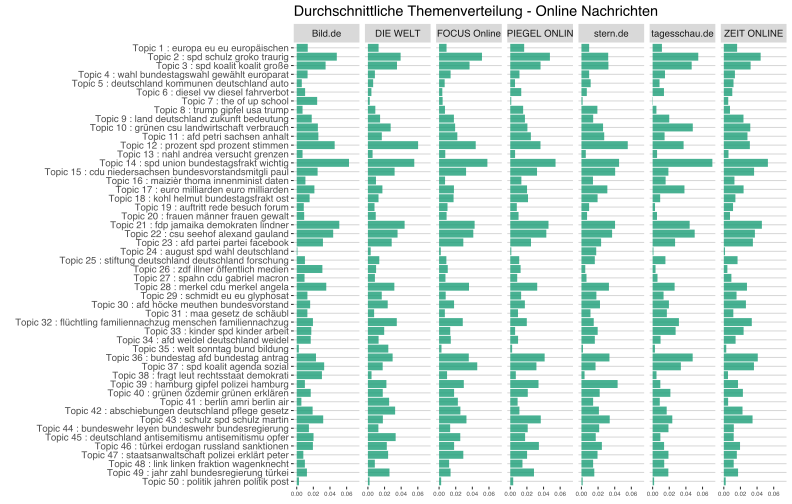
\includegraphics{agendaBias2_files/figure-latex/unnamed-chunk-16-1.pdf}

Again, to measure the bias and not just outlet specificities, for each
outlet the mean agenda selectivity of all other parties was subtracted
from each party's specific agenda selectivity value and then
standardized to range from −1 to 1, where −1 stands for both agendas
being not congruent at all and +1 stands for both agendas being
identical.

\begin{Shaded}
\begin{Highlighting}[]
\NormalTok{correlations <-}\StringTok{ }\NormalTok{correlations }\OperatorTok
\StringTok{  }\KeywordTok{group_by}\NormalTok{(medium) }\OperatorTok
\StringTok{  }\KeywordTok{mutate}\NormalTok{(}\DataTypeTok{avg_cor =} \KeywordTok{mean}\NormalTok{(cor)) }\OperatorTok
\StringTok{  }\KeywordTok{ungroup}\NormalTok{() }\OperatorTok
\StringTok{  }\KeywordTok{mutate}\NormalTok{(}\DataTypeTok{agenda_bias =}\NormalTok{ cor}\OperatorTok{-}\NormalTok{avg_cor,}
         \DataTypeTok{agenda_bias_norm =} \KeywordTok{normalize_data2}\NormalTok{(agenda_bias)}
\NormalTok{         )}
\end{Highlighting}
\end{Shaded}

\begin{Shaded}
\begin{Highlighting}[]
\KeywordTok{ggplot}\NormalTok{(correlations, }\KeywordTok{aes}\NormalTok{(party, agenda_bias_norm)) }\OperatorTok{+}
\StringTok{  }\KeywordTok{geom_col}\NormalTok{() }\OperatorTok{+}
\StringTok{  }\KeywordTok{coord_flip}\NormalTok{() }\OperatorTok{+}
\StringTok{  }\NormalTok{ggthemes}\OperatorTok{::}\KeywordTok{theme_igray}\NormalTok{() }\OperatorTok{+}
\StringTok{  }\KeywordTok{facet_wrap}\NormalTok{(}\OperatorTok{~}\NormalTok{medium) }\OperatorTok{+}
\StringTok{  }\KeywordTok{labs}\NormalTok{(}\DataTypeTok{x =} \OtherTok{NULL}\NormalTok{, }\DataTypeTok{y =} \OtherTok{NULL}\NormalTok{, }\DataTypeTok{title =} \StringTok{"Agenda bias"}\NormalTok{,}
       \DataTypeTok{subtitle =} \StringTok{"−1: agendas not congruent at all}\CharTok{\textbackslash{}n}\StringTok{+1: agendas are identical"}\NormalTok{)}
\end{Highlighting}
\end{Shaded}

\begin{verbatim}
## Warning in grid.Call(C_textBounds, as.graphicsAnnot(x$label), x$x,
## x$y, : Konvertierungsfehler für '−1: agendas not congruent at all' in
## 'mbcsToSbcs': Punkt ersetzt <e2>
\end{verbatim}

\begin{verbatim}
## Warning in grid.Call(C_textBounds, as.graphicsAnnot(x$label), x$x,
## x$y, : Konvertierungsfehler für '−1: agendas not congruent at all' in
## 'mbcsToSbcs': Punkt ersetzt <88>
\end{verbatim}

\begin{verbatim}
## Warning in grid.Call(C_textBounds, as.graphicsAnnot(x$label), x$x,
## x$y, : Konvertierungsfehler für '−1: agendas not congruent at all' in
## 'mbcsToSbcs': Punkt ersetzt <92>
\end{verbatim}

\begin{verbatim}
## Warning in grid.Call(C_textBounds, as.graphicsAnnot(x$label), x$x,
## x$y, : Konvertierungsfehler für '−1: agendas not congruent at all' in
## 'mbcsToSbcs': Punkt ersetzt <e2>
\end{verbatim}

\begin{verbatim}
## Warning in grid.Call(C_textBounds, as.graphicsAnnot(x$label), x$x,
## x$y, : Konvertierungsfehler für '−1: agendas not congruent at all' in
## 'mbcsToSbcs': Punkt ersetzt <88>
\end{verbatim}

\begin{verbatim}
## Warning in grid.Call(C_textBounds, as.graphicsAnnot(x$label), x$x,
## x$y, : Konvertierungsfehler für '−1: agendas not congruent at all' in
## 'mbcsToSbcs': Punkt ersetzt <92>
\end{verbatim}

\begin{verbatim}
## Warning in grid.Call(C_textBounds, as.graphicsAnnot(x$label), x$x,
## x$y, : Konvertierungsfehler für '−1: agendas not congruent at all' in
## 'mbcsToSbcs': Punkt ersetzt <e2>
\end{verbatim}

\begin{verbatim}
## Warning in grid.Call(C_textBounds, as.graphicsAnnot(x$label), x$x,
## x$y, : Konvertierungsfehler für '−1: agendas not congruent at all' in
## 'mbcsToSbcs': Punkt ersetzt <88>
\end{verbatim}

\begin{verbatim}
## Warning in grid.Call(C_textBounds, as.graphicsAnnot(x$label), x$x,
## x$y, : Konvertierungsfehler für '−1: agendas not congruent at all' in
## 'mbcsToSbcs': Punkt ersetzt <92>
\end{verbatim}

\begin{verbatim}
## Warning in grid.Call(C_textBounds, as.graphicsAnnot(x$label), x$x,
## x$y, : Konvertierungsfehler für '−1: agendas not congruent at all' in
## 'mbcsToSbcs': Punkt ersetzt <e2>
\end{verbatim}

\begin{verbatim}
## Warning in grid.Call(C_textBounds, as.graphicsAnnot(x$label), x$x,
## x$y, : Konvertierungsfehler für '−1: agendas not congruent at all' in
## 'mbcsToSbcs': Punkt ersetzt <88>
\end{verbatim}

\begin{verbatim}
## Warning in grid.Call(C_textBounds, as.graphicsAnnot(x$label), x$x,
## x$y, : Konvertierungsfehler für '−1: agendas not congruent at all' in
## 'mbcsToSbcs': Punkt ersetzt <92>
\end{verbatim}

\begin{verbatim}
## Warning in grid.Call(C_textBounds, as.graphicsAnnot(x$label), x$x,
## x$y, : Konvertierungsfehler für '−1: agendas not congruent at all' in
## 'mbcsToSbcs': Punkt ersetzt <e2>
\end{verbatim}

\begin{verbatim}
## Warning in grid.Call(C_textBounds, as.graphicsAnnot(x$label), x$x,
## x$y, : Konvertierungsfehler für '−1: agendas not congruent at all' in
## 'mbcsToSbcs': Punkt ersetzt <88>
\end{verbatim}

\begin{verbatim}
## Warning in grid.Call(C_textBounds, as.graphicsAnnot(x$label), x$x,
## x$y, : Konvertierungsfehler für '−1: agendas not congruent at all' in
## 'mbcsToSbcs': Punkt ersetzt <92>
\end{verbatim}

\begin{verbatim}
## Warning in grid.Call(C_textBounds, as.graphicsAnnot(x$label), x$x,
## x$y, : Konvertierungsfehler für '−1: agendas not congruent at all' in
## 'mbcsToSbcs': Punkt ersetzt <e2>
\end{verbatim}

\begin{verbatim}
## Warning in grid.Call(C_textBounds, as.graphicsAnnot(x$label), x$x,
## x$y, : Konvertierungsfehler für '−1: agendas not congruent at all' in
## 'mbcsToSbcs': Punkt ersetzt <88>
\end{verbatim}

\begin{verbatim}
## Warning in grid.Call(C_textBounds, as.graphicsAnnot(x$label), x$x,
## x$y, : Konvertierungsfehler für '−1: agendas not congruent at all' in
## 'mbcsToSbcs': Punkt ersetzt <92>
\end{verbatim}

\begin{verbatim}
## Warning in grid.Call(C_textBounds, as.graphicsAnnot(x$label), x$x,
## x$y, : Konvertierungsfehler für '−1: agendas not congruent at all' in
## 'mbcsToSbcs': Punkt ersetzt <e2>
\end{verbatim}

\begin{verbatim}
## Warning in grid.Call(C_textBounds, as.graphicsAnnot(x$label), x$x,
## x$y, : Konvertierungsfehler für '−1: agendas not congruent at all' in
## 'mbcsToSbcs': Punkt ersetzt <88>
\end{verbatim}

\begin{verbatim}
## Warning in grid.Call(C_textBounds, as.graphicsAnnot(x$label), x$x,
## x$y, : Konvertierungsfehler für '−1: agendas not congruent at all' in
## 'mbcsToSbcs': Punkt ersetzt <92>
\end{verbatim}

\begin{verbatim}
## Warning in grid.Call.graphics(C_text, as.graphicsAnnot(x$label), x$x,
## x$y, : Konvertierungsfehler für '−1: agendas not congruent at all' in
## 'mbcsToSbcs': Punkt ersetzt <e2>
\end{verbatim}

\begin{verbatim}
## Warning in grid.Call.graphics(C_text, as.graphicsAnnot(x$label), x$x,
## x$y, : Konvertierungsfehler für '−1: agendas not congruent at all' in
## 'mbcsToSbcs': Punkt ersetzt <88>
\end{verbatim}

\begin{verbatim}
## Warning in grid.Call.graphics(C_text, as.graphicsAnnot(x$label), x$x,
## x$y, : Konvertierungsfehler für '−1: agendas not congruent at all' in
## 'mbcsToSbcs': Punkt ersetzt <92>
\end{verbatim}

\includegraphics{agendaBias2_files/figure-latex/unnamed-chunk-18-1.pdf}

This underlines the importance of studying all three types of media
biases simultane- ously, as examining just one aspect provides a
misleading picture of the extent and nature of bias. The existence of
various and diverse forms of media bias also means that it is worth
considering their distinct effects on party preferences.


\end{document}
